\documentclass[tikz,convert={outfile=fonctions.png}]{standalone}

    \usepackage[utf8]{inputenc}
    \usepackage[europeanresistors]{circuitikz}

\begin{document}
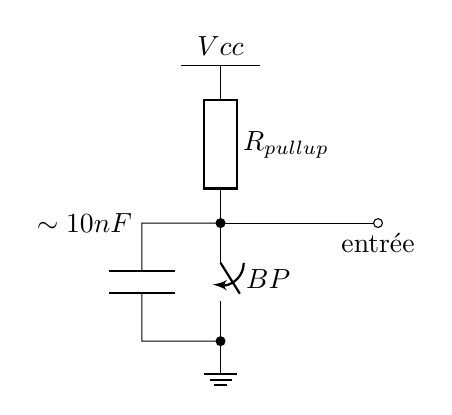
\begin{tikzpicture}[>=latex]

    \draw (-.5,4) -- node[anchor=south] {$Vcc$} (.5,4);

    \draw (0,4) to[R=$R_{pullup}$, -*] (0,2) to[cspst=$BP$, -*] (0,.5) node[ground] {};
\draw (0,2) -- (-1,2) node[left] {$\sim10nF$} to[C] (-1,.5) -- (0,.5);

    \draw (0,2) to[short, -o] (2,2) node[anchor=north] {entrée};

   
\end{tikzpicture}
\end{document}

